\documentclass[a4paper]{article}
\usepackage[warn]{mathtext}
\usepackage[utf8]{inputenc}
\usepackage[T2A]{fontenc}
\usepackage[english,russian]{babel}
\usepackage{booktabs}
\usepackage{multicol}
\usepackage{fancyhdr}
\usepackage{graphicx}
\usepackage{microtype}
\usepackage{wrapfig}
\usepackage{amsmath}
\usepackage{floatflt}
\usepackage{geometry} \geometry{verbose,a4paper,tmargin=2cm,bmargin=2cm,lmargin=1.5cm,rmargin=1.5cm}
\usepackage{float}
\usepackage{amssymb}
\usepackage{caption}
\usepackage{epsfig}
\usepackage{newunicodechar}

\begin{document}

\graphicspath{ {pictures/} }
\begin{center}
    {\scshape\Large Лабораторная работа по твердотельной электронике} \par

    \

    {\huge\bfseries № 12. Определение петли гистерезиса ферромагнетика магнитооптическим методом} \par 

    \

    {\large Яромир Водзяновский Б04-855а}
\end{center}

\

\
\textbf{Цель работы:} \par 
\begin{enumerate}
    \item Ознакомление с принципами применения магнитооптических методов для исследования прозрачных магнетиков. 
    \item Определение магнитных параметров исследуемого образца (коэрцетивная сила, поле насыщения)
    \item Изучение оснорв и принципов применения вычислительной техники для организации  автоматизированного сбора и анализа данных физического эксперимента
\end{enumerate}

\section{Теория}

Магнетизм - универсальное явление. Вещества со слабыми магнитными св-ми - пара- и диамагнетики, и с сильными - ферро- и ферримагнетики. \par 
У парамагнетиков отдельные атомы имеют свойц магн. момент, тепловое взаимодействие дизореинтирует их, а внешнее магнитное поле частично упорядочивает их. $\chi > 0$ \par 
У диамагнетиков собственный магн. момент равен нулю, однако направлен в противополжном напрвлении внешнему магнитному полю. $\chi < 0$. \par 
У сильных магнетиков внутренние взаимодействия приводят к пареллельной ориентации магнитных моментов отдельных атомов. Внешнее поле может ориентировать в одном направлении векторы отдельных областей - доменов. \par 
$$B = H + 4 \pi I$$
Формула связывает магнитную проницаемость с магнитной воспримчивостью. 
$$\mu = I + 4 \pi \chi$$
$I_R$ - остаточная намагнитченность. Поле $H_c$ - коэрцитивная сила, которой достаточно приложить в обратном напрвлении, чтобы убрать остаточную намагниченность. \par 
В ферромагнетике имеется только одна магнитная подрешетка, которая совпадает с кристаллической. В антиферромагнетике - две и более. Доменная структура образуется в магнетике за счет более слабых энергетических 
взаимодействий по сравнению с обменными. Основной причиной является стремление уменьшения вклада магнитостатической энергии, возникающей благодаря выходу нормальной составляющей намагниченности на поверхности  образаца.  \par 

Процесс намагничивания ферромагнетика различен в зависимости от величниы поля $H$. В слабых полях кривая имеет крутой подьем, соответствующим большим значениям восприимчивости, в сильных полях  кривая пологая. \par  
В слабых полях процесс есть рост магнитного момента одних областей за счет уменьшения других. В сильных полях поворачивается магнитный момент к направлению поля. \par 

При небольшом смещении доменной стенки параллельно самой себе на $\Delta X$ увеличение свободной энергии: 
$$2 H_c M_s L D \Delta X = \Delta(e_wLD)$$
$e_w$ - энергия доменной границы на деиничную площадь ее поверхности. 



\section{Эксперимент}

\begin{figure}[H]
    \begin{center}
        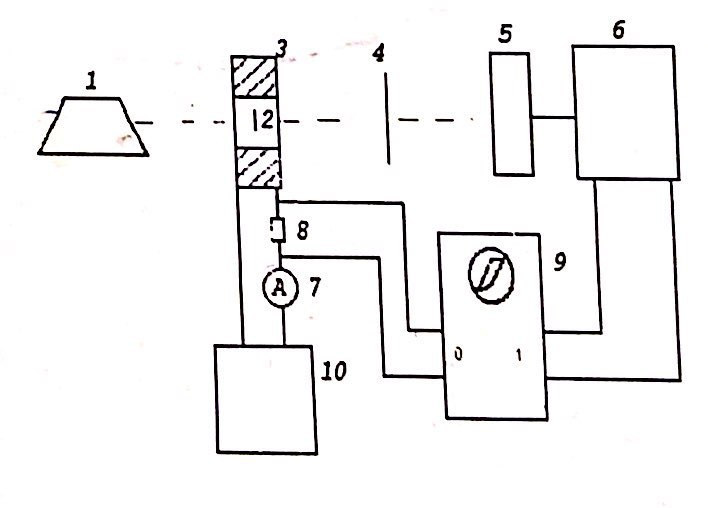
\includegraphics[scale=0.3]{setup.jpg}
        \caption{Схема установки. 1 - лазер, 2 - образец, 3 - катушка, 4 - анализатор, 5 - фотоприемник, 6 - усилитель, 7 - амперметр, 8 - резистор, 9 - виртуальный осциллограф.}
        \label{setup}
    \end{center}
\end{figure}

Блок-схема установки изображена на рис. \ref{setup}. Линейно поляризованное излучение лазера проходит через прозрачный исследуемый образец, анализатор и попадает на фотоприемкник, 
где преобразуется в электрический сигнал. Этот сигнал усиливается усилителем и подается на вход 1 осциллографа. Образец помещается в катушку. Переменный ток от источника питания подается через сопротивление на катушку. 
Напряжение, снимаемое с сопротивления подается на вход 0 осциллографа - сигнал пропорционланый велиине магнитного поля в катушке. \par 

Сигнал попадающий на вход 1 осциллографа?
$$I = I_0 \cos^2{(\gamma + \Psi_0 \sin{\omega t})}$$ 

$\Psi_0$ - величиная Фарадеевского вращения, $\omega$ - частота переменного напряжения.

$$U \sim 2 \sin{(2 \gamma)} \Psi_0 \sin{(\omega t)}$$
Амплитуда сигнала 1 пропорциональна величине фарадеевского вращения, которая пропорциональна проектции намагниченности образца на напрваление распространение света. 

\section{Ход работы}

\begin{enumerate}
    \item Соберем установку по рис. \ref{setup} и включим ее
    \item Определим оптимальное сопротивление резистора для подключения виртулаьного осциллографа. \par 
        $$R = \frac{I}{\sqrt{2} V} = \frac{1.75}{\sqrt{2} 5} = 0.24 \Omega$$
    \item Получим изображение петли на экране. Величина по горизонтальной оси - пропорциональна напряженности $H = \beta \frac{U}{R}$, где $\beta = 150$ Э/А. \par 
        По вертикали отнормируем значение по максимальному значению.
        \begin{figure}[H]
            \begin{center}
                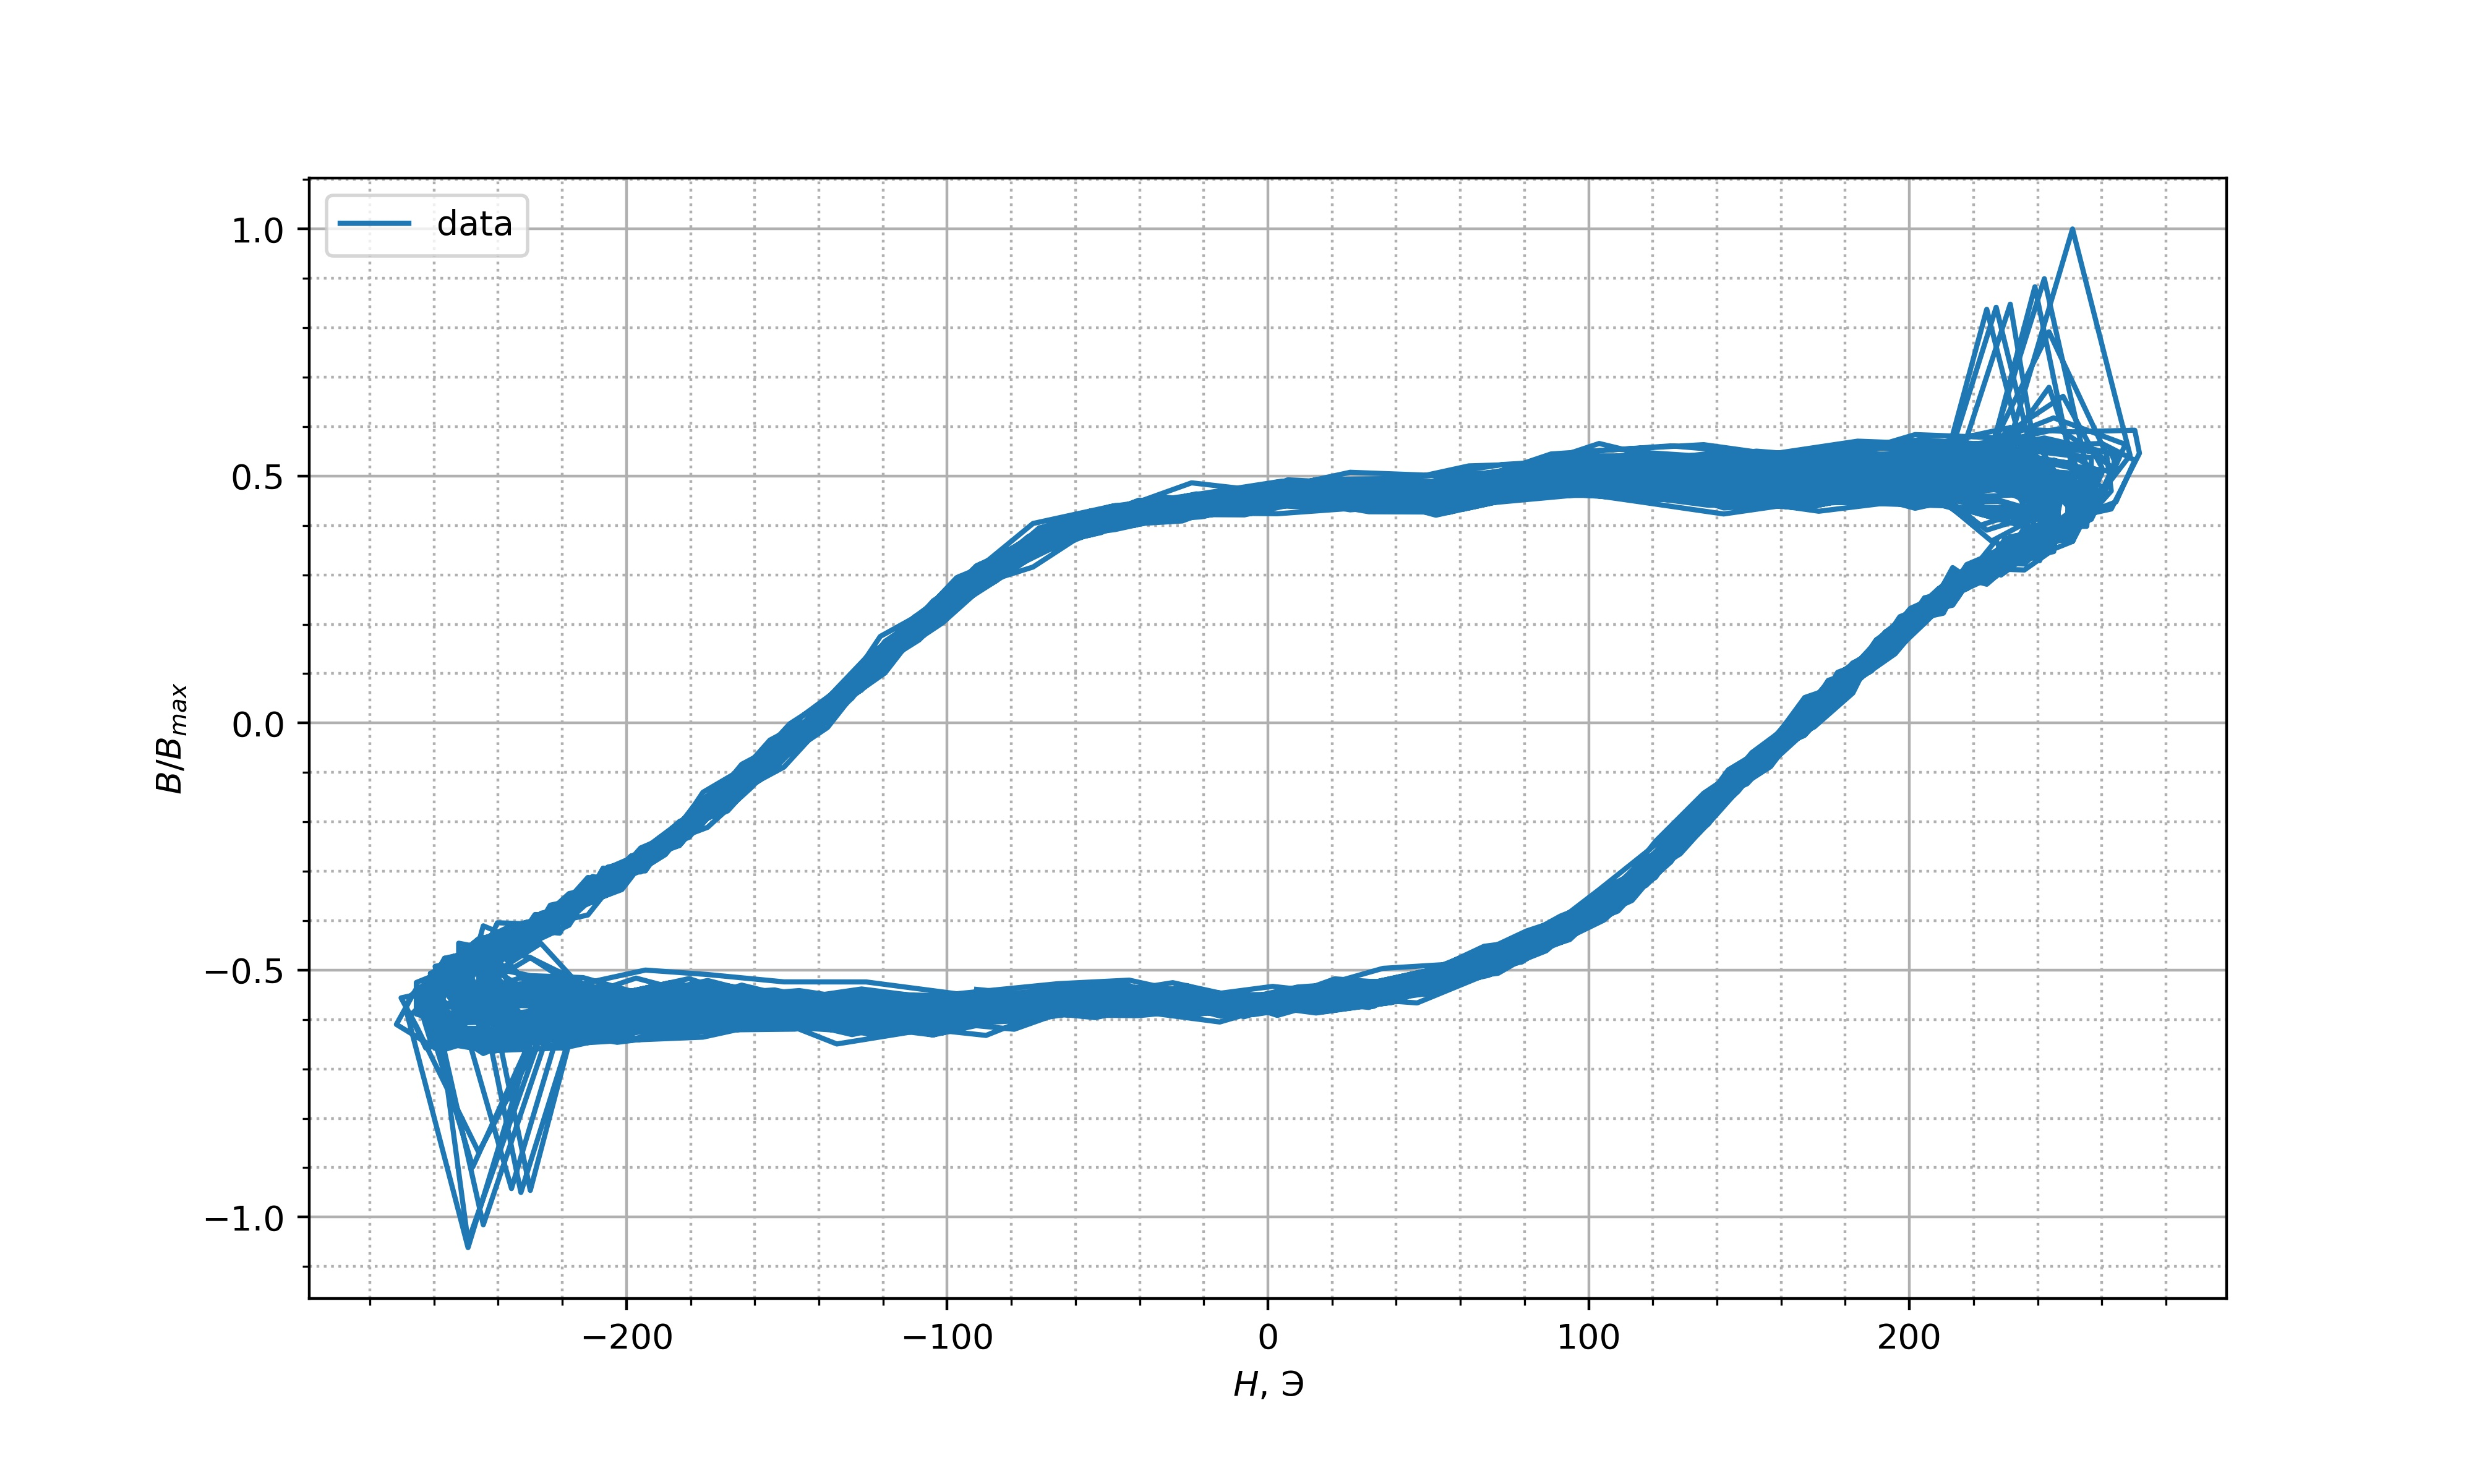
\includegraphics[scale=0.7]{gr1.jpg}
                \caption{}
                \label{gr1}
            \end{center}
        \end{figure}

    Откуда получим $H_c \approx 110$ Э, $H_s \approx 290$ Э.

\end{enumerate}

\section{Вывод}

В ходе работы был изучен принцип магнитооптического метода исследования прозрачных магнетиков. С его помощью построена петля гистерезиса исследуемого образца, а также определены его некоторые магнитные параметры, в частности коэрцитивная сила ($H_c \approx 110$ Э) и поле насыщения ($H_s \approx 290$ Э). Также в работе были изучены основы применения электронной вычислительной техники для автоматизированного сбора и анализа экспериментальных данных.


\section{Ответы на вопросы}

\begin{enumerate}
    \item \textbf{Какие факторы обуславливают наличие петли гистерезиса у ферроматгнитных материалов?} \par 
    Гистерезис (запаздывание) происходит потому, что перестройка структуры доменов сопровождается потерей
    энергии и требуется обратная сила (Hc), чтобы вернуть домены в исходное состояние.
    \item \textbf{Какие физические принципы лежать в основе работы экспериметальной установки?}  \par 
        Закон Маллюса, эффект Фарадея, гистерезис ферромагнетика.
    \item \textbf{Что такое "коэрцитивность" и от чего она зависит?}  \par 
        Коэрцитивная сила - необходимая сила чтобы вернуть домены в исходное состояние. Коэрцитивная сила сильно зависит от текстурованности материала, режима его термообработки, направления намагничивающего поля для текстурованных и анизотропных материалов, поэтому в таблице для некоторых материалов приведены диапазоны изменения коэрцитивной силы. 
    \item \textbf{Какова природа магнитных св-в ферромагнетиков?}  \par 
    В ферромагнетиках ответственными за их магнитные свойства являются собственные (спиновые) магнитные моменты электронов. Атомы ферромагнетика объединяются в группы размером около 1мкм, называемые доменами. В пределах домена магнитные моменты атомов
    параллельны друг другу, а намагниченности разных
    доменов отличаются по направлению. Так как в смежных
    доменах эти направления различны, то в целом
    намагниченность образца магнетика нулевая.
    Образование доменов обусловлено тем, что в таком
    состоянии суммарная энергия атомов образца
    минимальна, и это состояние, следовательно, является
    наиболее энергетически выгодным. Под влиянием
    внешнего поля происходит смещение доменных стенок,
    растут те домены, намагниченность которых направлена вдоль H. Происходит также поворот направления намагниченности доменов в сторону внешнего поля.
    \item \textbf{Чем отличаются процессы намагничивания ферромагнетиков, парамагнетиков, диамагнетиков?}  \par  
    У парамагнетиков отдельные атомы имеют свойц магн. момент, тепловое взаимодействие дизореинтирует их, а внешнее магнитное поле частично упорядочивает их. $\chi > 0$ \par 
    У диамагнетиков собственный магн. момент равен нулю, однако направлен в противополжном напрвлении внешнему магнитному полю. $\chi < 0$. \par 
    У ферромагнетиков внешнее поле может ориентировать в одном направлении векторы отдельных областей - доменов. Намагничивание имеет необратимый характер, тк смещаются доменные границы, а также вращается $\vec{I}$.   
    \item \textbf{Что такое "доменная структура" и каковы причины ее образования?}  \par 
    Доменная структура - комплекс областей со спонтанной однородной намагниченностью. \par 
    Ландау и Лифшиц показали, что образование доменной структуры является следствием конкуренции нескольких вкладов в полную энергию ферромагнетика. А именно, 1) - обменной энергии - $U_{обм}$, 2) - энергии кристаллографической анизртропии - $U_K$, 3) - энергия магнитострикционной деформации - $U_{\lambda}$, 4) - магнитоупругой энергии $U_{\sigma}$ , 5) - магнитостатической энергии - $U_0$, 6) - магнитной энергии - $U_M$.
    \item \textbf{Что такое "доменная границы" и от чего зависит ее удельная энергия и толщина?}  \par
        Граница - область с плавным разворотом вектора намагниченности от направления в одном домене к напрвлению вектора намагниченности в сосднем домене. \par 
        Энергия зависит от обменной константы и константы одноосной анизотропии. \par 
        Ширина доменной стенки изменяется из-за двух противоположных энергий, которые ее создают: энергия магнитокристаллической анизотропии и энергия обмена, оба из которых имеют тенденцию быть как можно более низкими, чтобы находиться в более благоприятном энергетическом состоянии. Энергия анизотропии является самой низкой, когда отдельные магнитные моменты выровнены по осям кристаллической решетки, что уменьшает ширину доменной стенки. И наоборот, обменная энергия уменьшается, когда магнитные моменты выровнены параллельно друг другу, и, таким образом, толщина стенки увеличивается из-за отталкивания между ними (когда антипараллельное выравнивание сближает их, работая для уменьшения толщины стенки).
\end{enumerate}

\end{document}